\section{Implications for the study of \ac{WCA} footprints}\label{sec:implications:footprint}

% \subsection{Application lifetimes}

We begin by studying the implications of such a model on the estimation of application footprints as described by their lifetimes.
In the context of \ac{WCA}, we will understand \emph{application lifetime} as the time it takes a user to complete a specified task.
This is an important metric for \ac{WCA} optimization, as it directly relates to system resource utilization and contention, and to energy consumption.

In order to illustrate the consequences of using a less realistic model which does not take into account higher order effects, we introduce here a reference model to which we will compare our more realistic models.
This new model represents a first-order approximation to empirical execution time modeling, and consist simply of an \ac{exGaussian} distribution fitted to all execution time samples collected for \textcite{olguinmunoz:impact2021}.
This distribution is then randomly sampled at runtime to obtain execution times for each step, without any sort of adjustment to the current state of the system.

We start by studying application lifetimes in a controlled, ideal setup by using the timing models to generate execution times for sequences of \num{100} steps subject to constant \acp{TTF}.
These runs are completely simulated and no sampling of video frames is performed; for each step, we simply feed the models a predefined \ac{TTF} and record the generated execution time.
We use the combination of \acp{TTF} and execution times to calculate theoretical step duration times and subsequent total application lifetimes.
This is done for \num{25} linearly distributed \acp{TTF} in the \SIrange[]{0}{5}{\second} range; \num{45} independent repetitions for each combination of model configuration and \ac{TTF}.

\begin{figure}
    \centering
    \begin{subfigure}[]{\columnwidth}
        \centering
        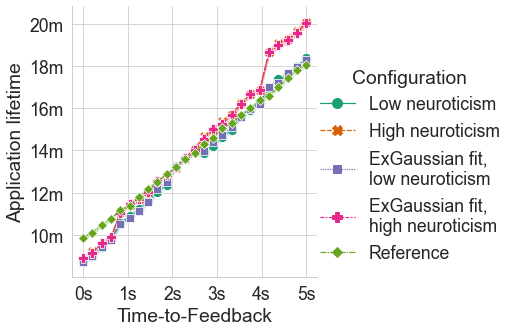
\includegraphics[width=\textwidth]{figs/new_model/lifetime_all_ttfs.png}
        \caption{%
            Evolution of mean application lifetimes as \acp{TTF} increase.
            Error bars indicate \SI{95}{\percent} \acp{CI}.
        }
    \end{subfigure}
    \begin{subfigure}[]{\columnwidth}
        \centering
        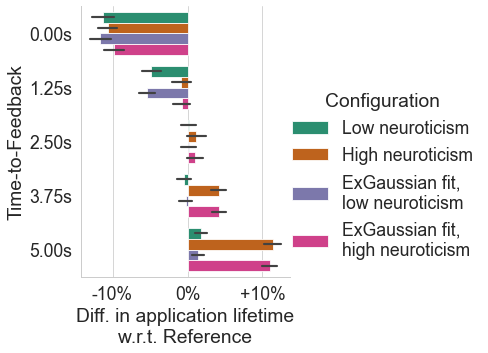
\includegraphics[width=\textwidth]{figs/new_model/lifetime_diff.png}
        \caption{%
            Percentage difference in mean application lifetimes with respect to the reference model at select \acp{TTF}.
            Error bars indicate the \SI{95}{\percent} \acp{CI}, calculated using a two-sided T-test.
        }
    \end{subfigure}
    \caption{\acl{TTF} versus application lifetime.}\label{fig:lifetimes}
\end{figure}

The results of this investigation are presented in \cref{fig:lifetimes}.
Compared to the reference model, our realistic model is, on average, roughly \SI{11}{\percent} faster when subject to low \acp{TTF}.
At higher \acp{TTF}, the behavior of the model depends on its level of normalized neuroticism.
At low neuroticism, the behavior of the realistic model results in total task durations that are basically indistinguishable from the reference model.
However, at high neuroticism, the model once again results in a considerable difference in total task duration with respect to the reference --- this time extending durations by \textasciitilde\SI{11}{\percent} on average.

\begin{figure}
    \centering
    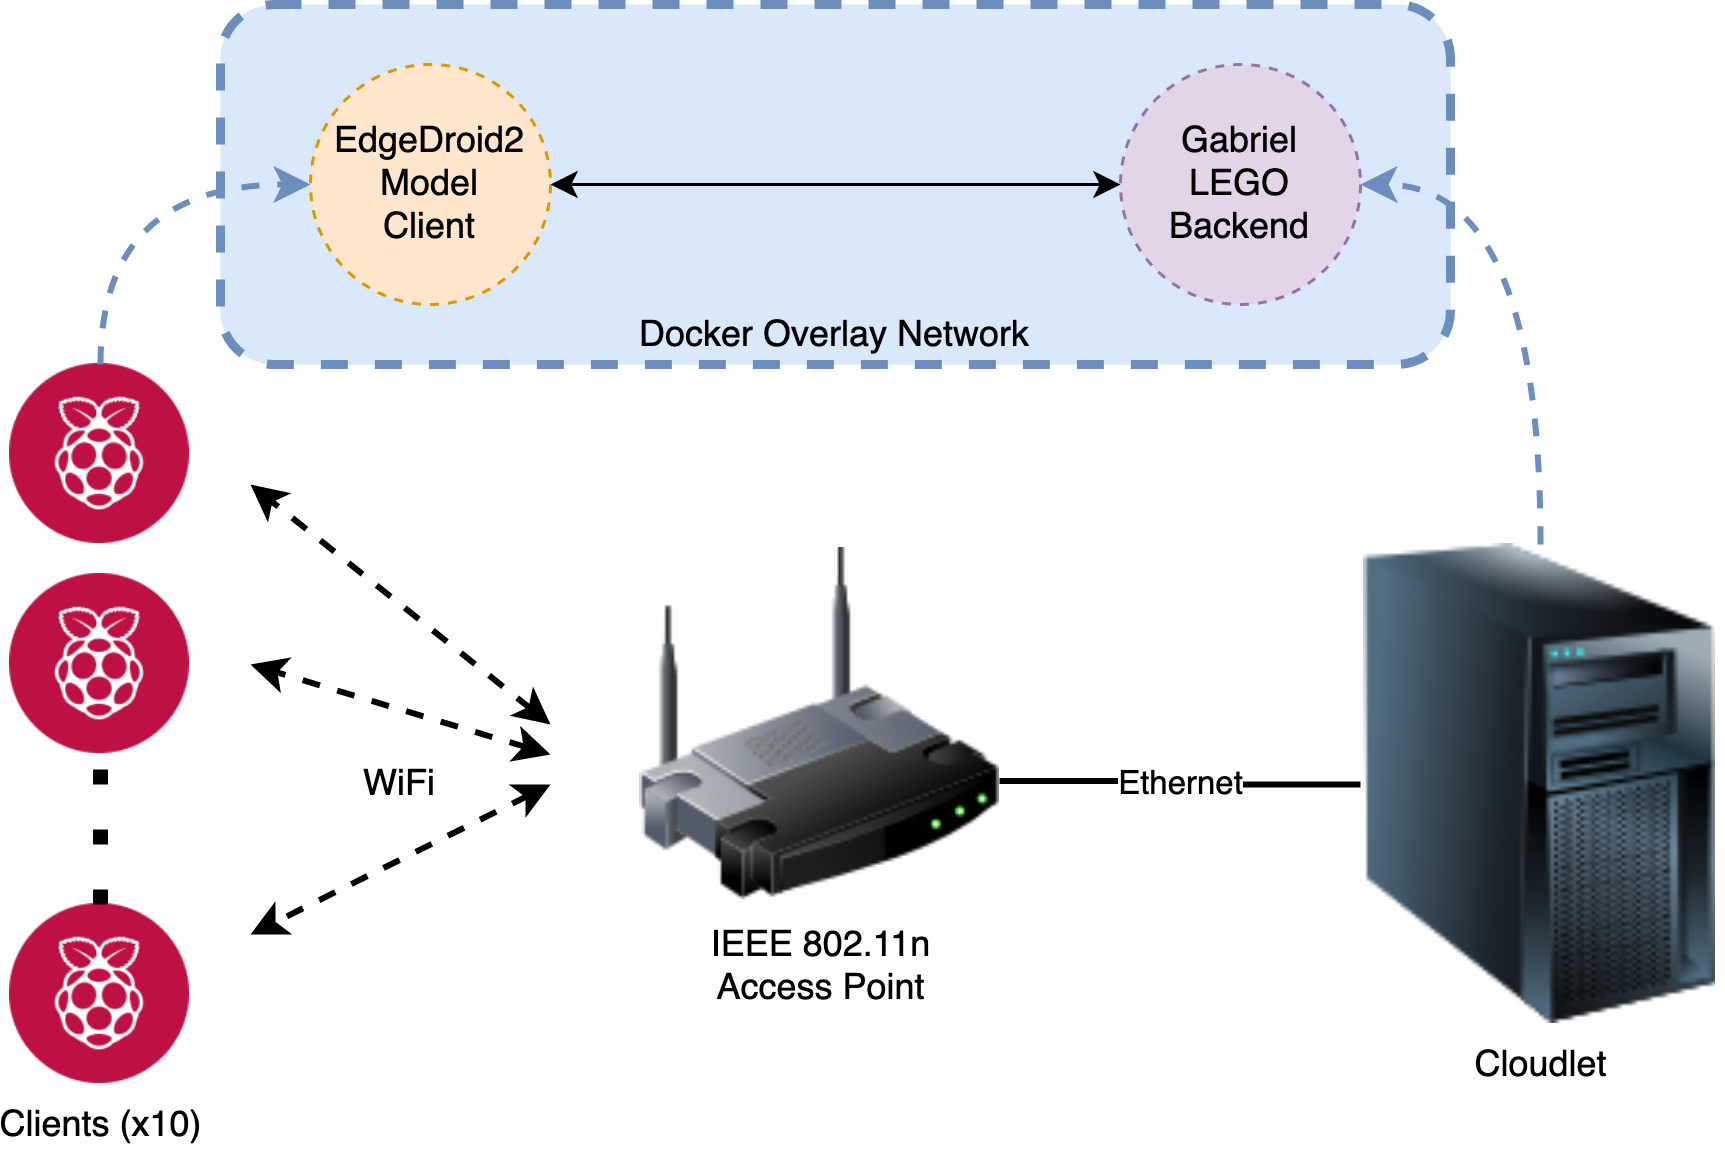
\includegraphics[width=\columnwidth]{figs/EdgeDroid2ExperimentalSetup.png}
    \caption{%
        Experimental setup used to study the implications of the realistic models of human behavior for \ac{WCA}.
        We deploy containerized instances of the client-server loop running the models on a testbed consisting of \num{10} Raspberry Pi clients connected to a cloudlet over a \acs*{COTS} \acs{IEEE} \num{802.11}b/g access point.
    }\label{fig:expsetup}
\end{figure}

Next we study the effects of first- versus second-order models in a more realistic setting.
The models, reference and realistic, are deployed on the Raspberry Pi clients of the testbed depicted in \cref{fig:expsetup}.
For this, the timing models and frame generator are integrated into a custom Python3 client for the Gabriel \ac{WCA} platform~\cite{Chen2018application}, which are then paired with real instances of Gabriel deployed on the cloudlet.
Clients and cloudlet communicate over an \acs{IEEE} \num{802.11}b/g wireless network.
Our choice of wireless standard is simply motivated by a desire to amplify the potential effects of network congestion.

\begin{figure}
    \centering
    \begin{subfigure}[]{\columnwidth}
        \centering
        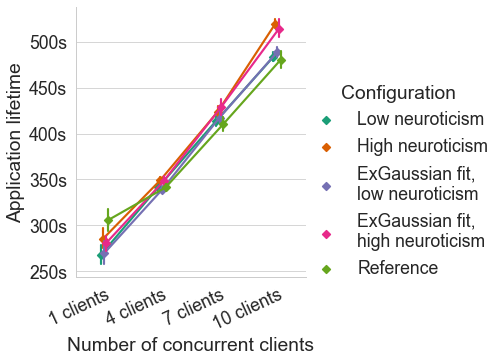
\includegraphics[width=\textwidth]{figs/new_model/lifetime_testbed.png}
        \caption{%
            Mean application lifetimes per testbed configuration.
            Note that due to the low number of samples, means have been calculated using the geometric instead of arithmetic average. 
            Error bars indicate \SI{95}{\percent} \acp{CI}, calculated using bootstrapping.
        }
    \end{subfigure}
    \par\bigskip
    \begin{subtable}{\columnwidth}
        \centering
        \begin{tabular}{lrrrr}
            \toprule
            \# clients & 1 & 4 & 7 & 10 \\
            \ac{RTT} & \SI{0.42}{\second} & \SI{1.12}{\second} & \SI{1.92}{\second} & \SI{2.68}{\second} \\
            \bottomrule
        \end{tabular}
        \caption{Mean measured \aclp{RTT} for each testbed configuration.}
    \end{subtable}
    \par\bigskip
    \begin{subfigure}[]{\columnwidth}
        \centering
        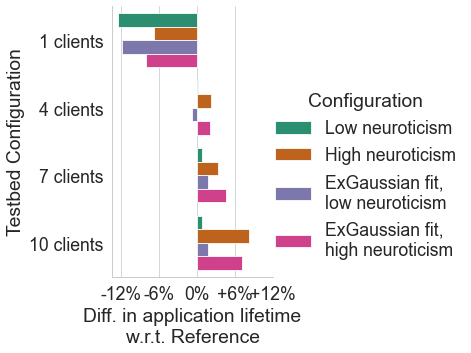
\includegraphics[width=\textwidth]{figs/new_model/lifetime_testbed_diff.png}
        \caption{%
            Percentage difference in mean application lifetimes with respect to the reference model.
            Confidence intervals have been omitted due to the low number of samples and the use of the geometric mean.
        }
    \end{subfigure}
    \caption{Application lifetimes in the realistic scenarios.}\label{fig:testbed_lifetimes}
\end{figure}

We deploy configurations running \num{45}-step versions of the LEGO task described in \textcite{olguinmunoz:impact2021}.
The testbed configurations include setups with \numlist{1;4;7;10} clients.
Due to having only limited time, each combination of testbed and timing model configuration is only repeated \num{10} times.
The results are presented in \cref{fig:testbed_lifetimes}.
Owing to the low number of samples, we opt here for the geometric rather than arithmetic mean to represent our results.
The results are nonetheless clear, and follow the same pattern as the previously discussed results under ideal, controlled circumstances.
With just a single client and mean \ac{RTT} of around \SI{400}{\milli\second}, all parameterizations of the realistic model achieved an average task duration \SIrange{6}{12}{\percent} shorter than the reference.
At \num{10} clients, the results mimic those at higher \acp{TTF} in the ideal controlled setup, with high neuroticism parameterizations reaching \textasciitilde\SI{8}{\percent} longer application lifetimes.

These results highlight the importance of accurate execution time modeling when studying \ac{WCA} application lifetimes.
Not only do we see considerable differences in lifetimes at relatively moderate levels of system congestion, but the sign of these differences depends on the load placed on the system.
Imagine thus a system designer studying resource consumption optimization in a \ac{WCA}.
If they were to employ the reference model for their study on an unimpaired system, it could lead them to significantly underestimate the potential for optimization of resource consumption, leaving performance (and, potentially, monetary) gains on the table.
On the other hand, under heavy load, they would instead underestimate system resource occupation, again leading to performance losses.

% \todo[inline]{%
%     Ergo we need a second order model. Everything that comes afterwards is only with second order model. Play with RTT.
% }


% .as well as an additional setup with \num{10} clients during which an instance of the \emph{iperf3}\footnote{\href{https://iperf.fr/}{https://iperf.fr/}} network load generator is also running on each client.
% The \emph{iperf3} instances each generate \SI{1.5}{Mbps} of upstream \ac{TCP} traffic, further congesting the wireless network.